%! TEX root=./main.tex

\lecture{15}{Week 8}{Floating Point}

\subsubsection{Floating-Point Rounding}
The basic idea of rounding is the first compute the exact result, then round it to make it fit into the desired precision.

There are four different rounding modes. All are acceptable IEEE standards, but in C we cannot change the mode without getting into Assembly.
\begin{itemize}
    \item Towards zero
    \item Round down ($-\infty$)
    \item Round up ($+\infty$)
    \item Nearest Even (default)
\end{itemize}

All modes, beside round-to-even are biased towards some systematic error. Round-to-even is statistically the most accurate one. It rounds the number in such a ways, that when we are half-way between two numbers, it rounds towards the even number. In all other cases, it rounds towards the closer number.

The following example show rounding to the nearest hundredth

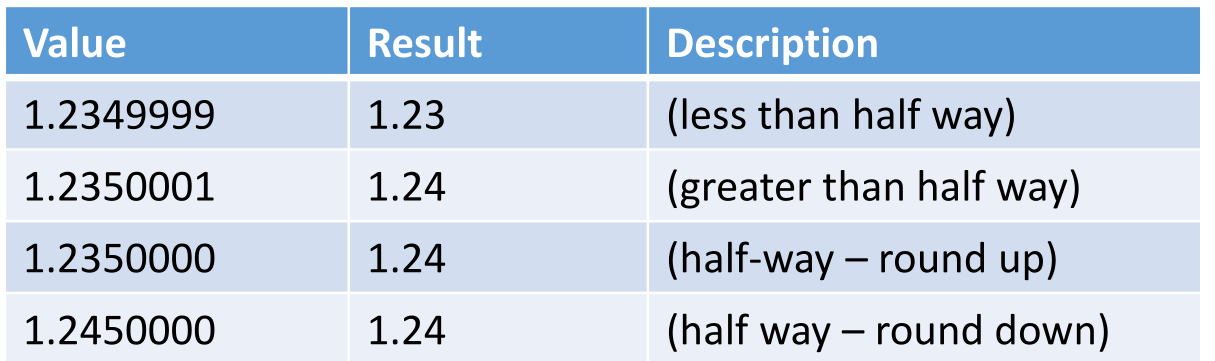
\includegraphics[width=0.8\textwidth]{15_roundtoevenexample.png}

When considering binary numbers we first notice that:
\begin{itemize}
    \item Number is even if LSB is $0$
    \item Number is half way between to numbers when the bits to the right of the rounding position are $100\dots _2$
\end{itemize}

In the following example we round towards the nearest $1/4$ ($2$ bit positions after the binary point)

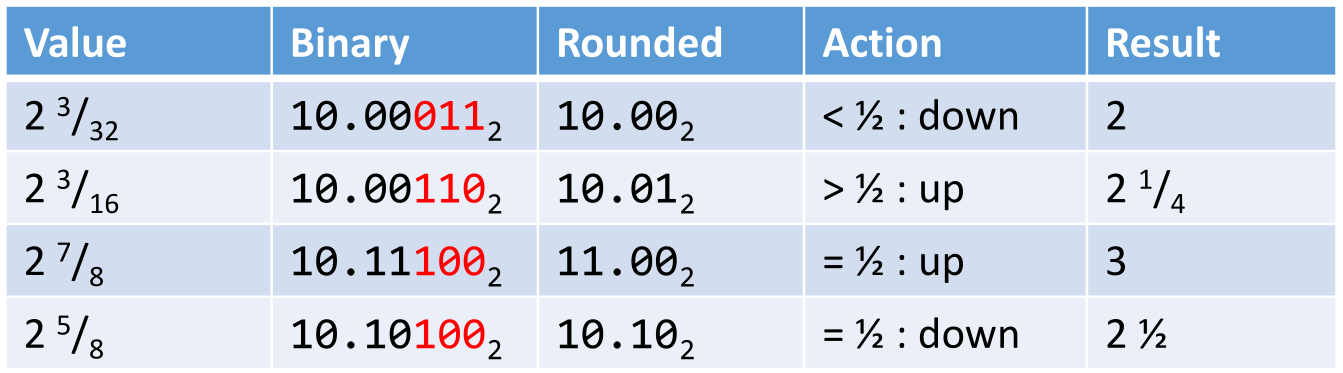
\includegraphics[width=0.8\textwidth]{15_roundtoevenexamplebinary.png}

Building circuits for rounding is rather easy.

\paragraph{Creating floating point number}
Before considering rounding in arithmetic in floating point notation, we have a look how to convert a given unsigned binary number into a floating point number. This comprises of the following steps:

\subparagraph{Normalize}
In the first step we make sure that the binary number is of the form $1.xxx\dots$. We drop all leading $0$ and shift the number to the left, while incrementing the exponent, till we have our desired format.

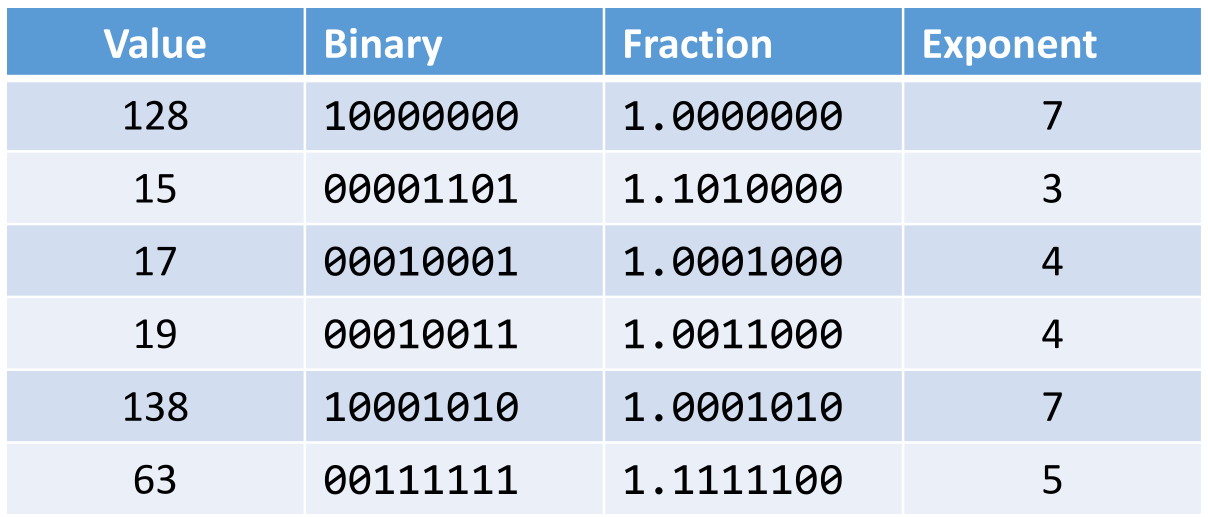
\includegraphics[width=0.8\textwidth]{15_fpexamplenormalize.png}

\subparagraph{Rounding}
Assume the frac bit of the floating point number has length $3$. Therefore, we have to round the fraction to three digits after the binary point. For that purpose we name the LSB which remains after rounding, the \textit{guard bit}, the MSB which gets remove the \textit{round bit}, and the \textit{sticky bit} is the OR of all other truncated bits.

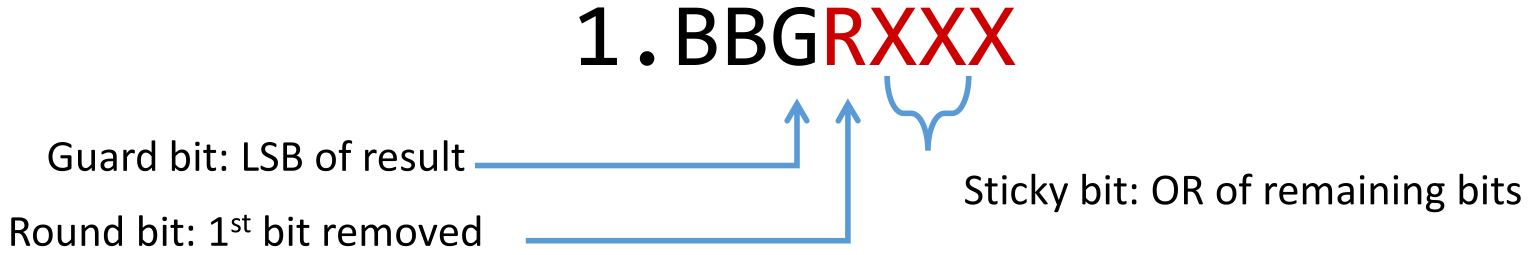
\includegraphics[width=0.8\textwidth]{15_fpexampleroundscheme.png}

The condition for the rounding are the following:
\begin{itemize}
    \item Round $=1$, Sticky $=1 \implies > 0.5$ (round up)
    \item Guard $=1$, Round $=1$, Sticky $= 0 \implies$ Round-to-even
\end{itemize}

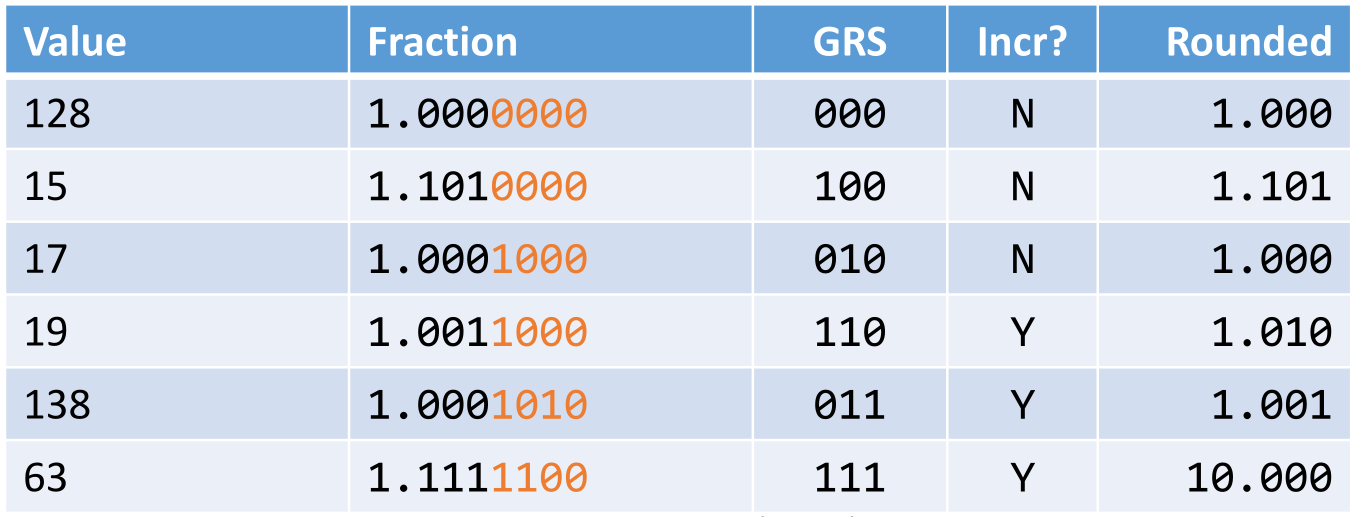
\includegraphics[width=0.8\textwidth]{15_fpexamplerounding.png}

\subparagraph{Postnormalize}
Rounding may cause overflow. We fix that by right-shifting once and increasing the exponent.

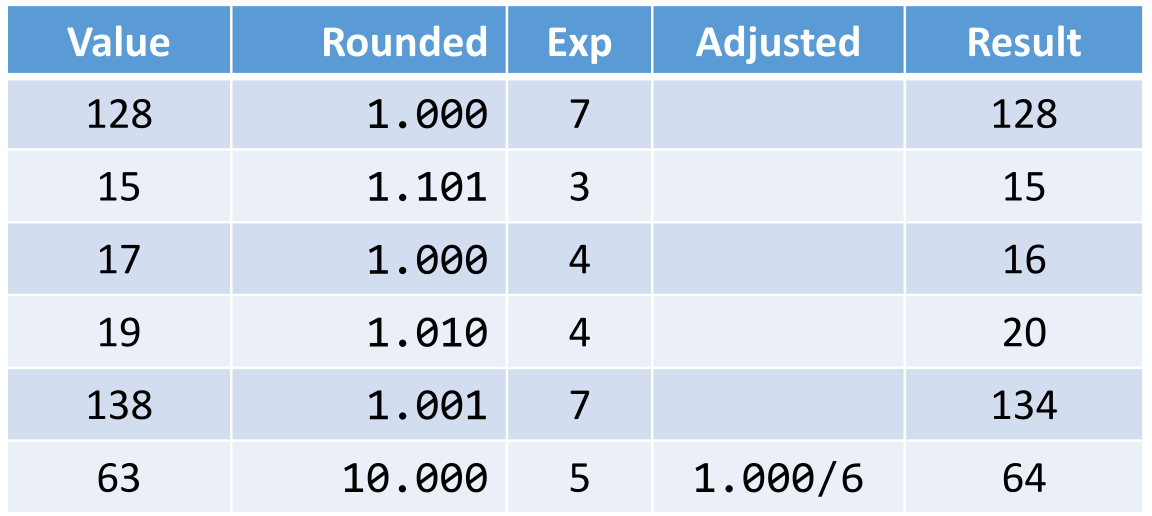
\includegraphics[width=0.8\textwidth]{15_fpexamplepostnormalize.png}

\subsubsection{Floating-Point Addition and Multiplication}
Given two number is FP notation $(-1)^{s1} M_1 2^{E1}$ and $(-1)^{s2} M_2 2^{E2}$:

\paragraph{Multiplication}
The result of the multiplication of the two numbers of $(-1)^s M 2^E$, where:
\begin{itemize}
    \item $\mathbf{s} = s_1 \land s_2$
    \item $\mathbf{M} = M_1 \cdot M_2$
    \item $\mathbf{E} = E_1 + E_2$
\end{itemize}

After the calculation, we have to consider a few cases:
\begin{itemize}
    \item If $M \ge 2$ (i.e. not of the form $1.xx\dots_2$), we shift $M$ right and increment $E$
    \item If $E$ out of range we overflow
    \item Round $M$ to find frac precision (as we did when converting unsigned int to FP notation)
\end{itemize}

\subparagraph{Properties}
\begin{itemize}
    \item Closed under multiplication: \textbf{Yes}
        \begin{itemize}
            \item May generate infinity or NaN
        \end{itemize}
    \item Commutative: \textbf{Yes}
    \item Associative: \textbf{No}
        \begin{itemize}
            \item Overflow and inexactness of rounding
        \end{itemize}
    \item $1$ is multiplicative identity: \textbf{Yes}
    \item Multiplicant distributes over addition: \textbf{No}
        \begin{itemize}
            \item Possibility of overflow and inexactness of rounding
        \end{itemize}
    \item Monotonicity: \textbf{Almost}
        \begin{itemize}
            \item Except for infinity and Nan
        \end{itemize}
\end{itemize}

\paragraph{Addition}
Addition is a little more complex than multiplication because the result can easily overflow. We assume that $E_1 > E_2$ and the result of the addition is $(-1)^s M 2^E$, where:
\begin{itemize}
    \item $\mathbf{s}$ and $\mathit{M}$ are the result of signed align and addition
    \item $\mathbf{E} = E_1$
\end{itemize}

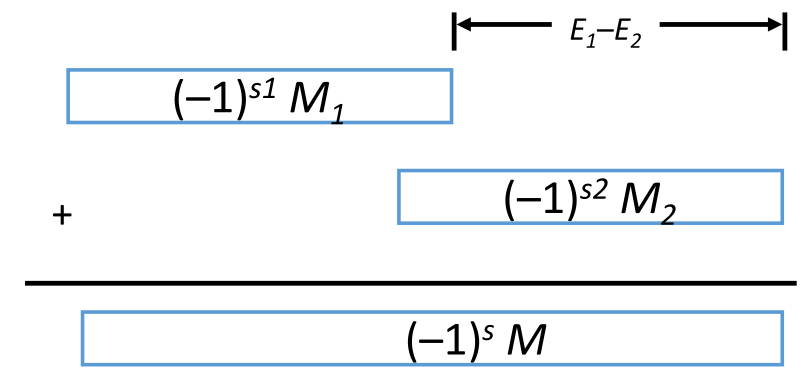
\includegraphics[width=0.8\textwidth]{15_fpaddition.png}

After the calculation, we have to consider a few cases:
\begin{itemize}
    \item If $M \ge 2$ (i.e. not of the form $1.xx\dots_2$), we shift $M$ right and increment $E$
    \item If $M <  1$ (i.e. not of the form $1.xx\dots_2$), we shift $M$ left and decrement $E$
    \item If $E$ out of range we overflow
    \item Round $M$ to find frac precision (as we did when converting unsigned int to FP notation)
\end{itemize}

\subparagraph{Properties}
\begin{itemize}
    \item Closed under addition: \textbf{Yes}
        \begin{itemize}
            \item May generate infinity or NaN
        \end{itemize}
    \item Commutative: \textbf{Yes}
    \item Associative: \textbf{No}
        \begin{itemize}
            \item Overflow and inexactness of rounding
        \end{itemize}
    \item $0$ is additive identity: \textbf{Yes}
    \item Every element has additive inverse: \textbf{Almost}
        \begin{itemize}
            \item Except for infinity and Nan
        \end{itemize}
    \item Monoticity: \textbf{Almost}
        \begin{itemize}
            \item Except for infinity and Nan
        \end{itemize}
\end{itemize}

Add smallest numbers first to get the most accurate result.


2/3 is float
2/3.0 is double (is is it the other way?)

\subsubsection{SSE Floating Point}
CPUs have designated modules for floating point arithmetic. In old architectures, the floating point unit was even placed on a different chip(co-processor). All x86-64 have SSE3 (streaming SIMD extension), which is a superset of SSE, and which supports single and double precision. This allows CPUs to conduct vector instructions, meaning, parallel operation on small (length $2-8$ byte) vectors of integers of floats. $n$-way means that a vector holds $n$ elements.

\paragraph{SSE3 Registers}
SSE3 provides an additional set of $16$ registers. They have each size of $128$ bits and can be used to store:
\begin{itemize}
    \item Integer Vector:
        \begin{itemize}
            \item $16$-way byte
            \item $8$-way $2$ bytes
            \item $4$-way $4$ bytes
        \end{itemize}
\end{itemize}

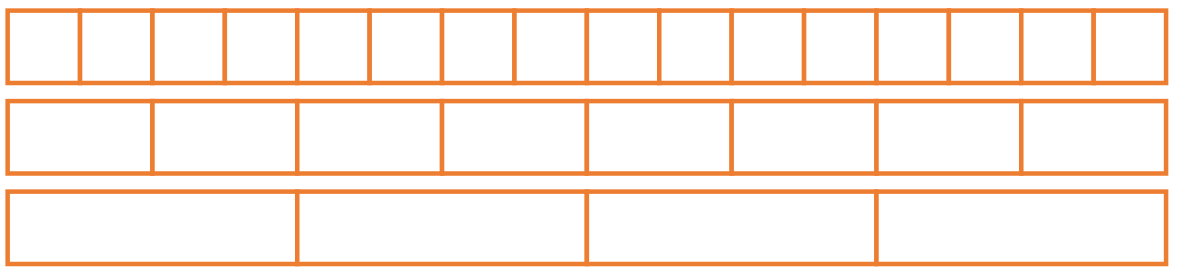
\includegraphics[width=0.8\textwidth]{15_sseregint.png}

\begin{itemize}
    \item Floating Point Vector:
        \begin{itemize}
            \item $4$-way single
            \item $2$-way double
        \end{itemize}
\end{itemize}

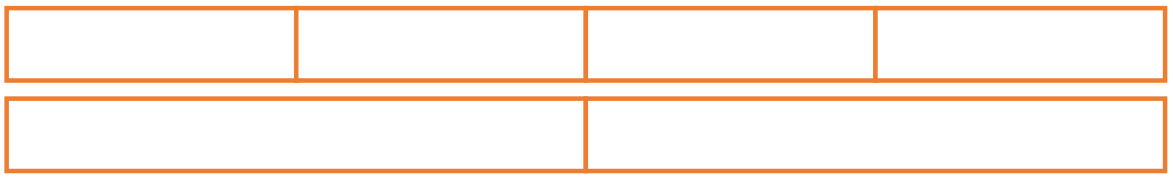
\includegraphics[width=0.8\textwidth]{15_sseregfloat.png}


\begin{itemize}
    \item Floating Point Scalars (not whole vector is used):
        \begin{itemize}
            \item single
            \item double
        \end{itemize}
\end{itemize}

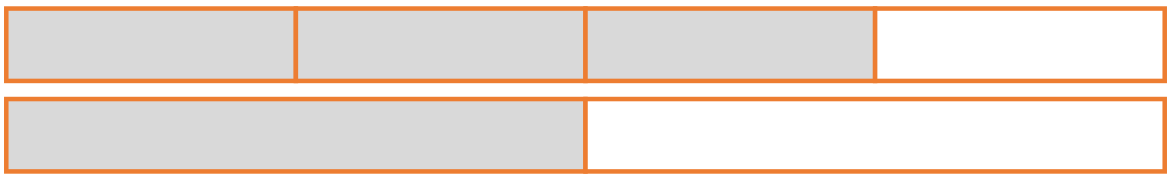
\includegraphics[width=0.8\textwidth]{15_ssescalar.png}

They are named \code{\%xmm0} through \code{\%xmm15} and they are all caller saved.

\paragraph{SSE3 Instructions}
Basic instruction names are composed of three parts:
\begin{itemize}
    \item The name of the instruction: \code{add, sub, mov} etc
    \item The format of the data: \code{p} for packed (vectors) and \code{s} for scalar
    \item The data type of the data: \code{s} for single precision and \code{d} for double precision
\end{itemize}

\subparagraph{Moves}
\code{movss}, \code{movsd} are used to move data from reg to reg, reg to mem or mem to reg.


\includegraphics[width=0.8\textwidth]{15_sseinstructionmove.png}

\subparagraph{Arithmetic}
There exist the following arithmetic instructions:

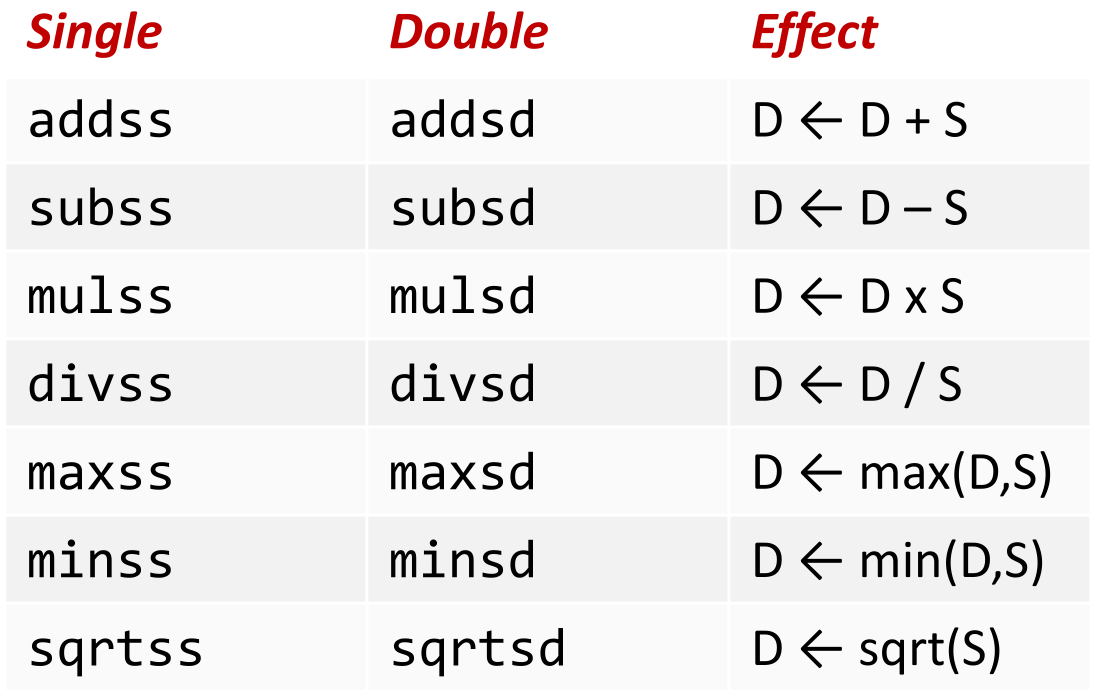
\includegraphics[width=0.8\textwidth]{15_instructionarithmetic.png}

\subparagraph{Concessions}
Are used to convert the type of data. Their format is a little more complicated.

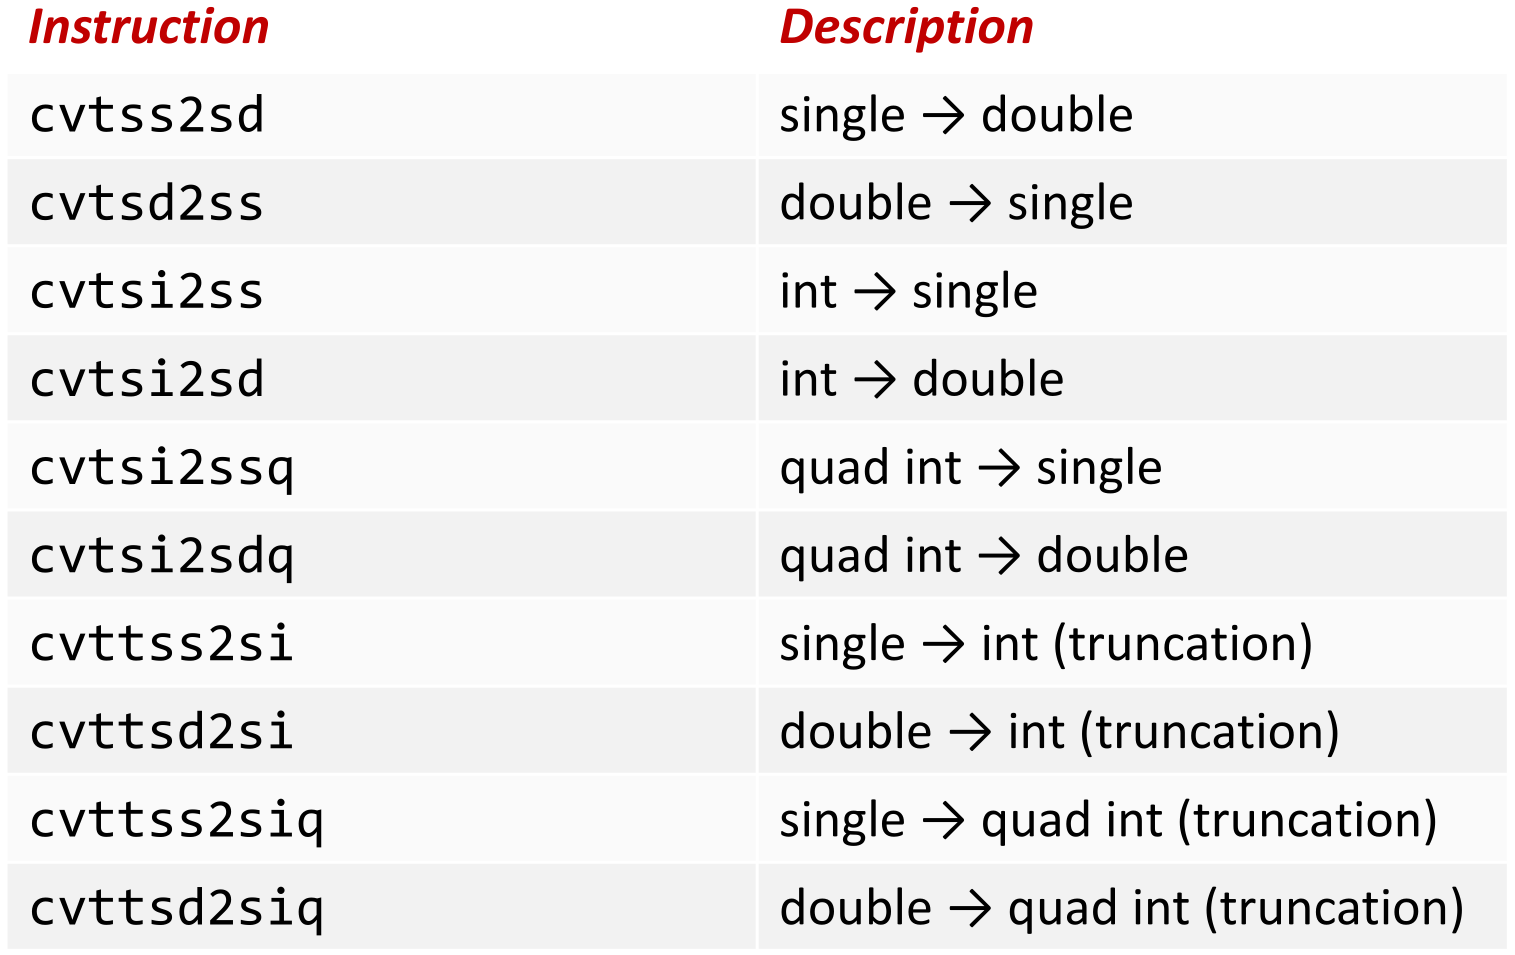
\includegraphics[width=0.8\textwidth]{15_sseinstructionconversions.png}

\paragraph{GCC and SSE3}
Since recently, gcc can try to to autovectorize given code. This functionality is very limited and does not guarantee any speed-up. C itself is poorly suited for writing vectorized code, i.e. code for GPUs. But there are dedicated languages for this purpose. Writing vectorized code is very hard but the key to performance.
